\newpage
% TODO: ТУТ ВСЕ НАДО ПОМЕНЯТЬ НА СВОЕ!!!
\section{Обработка результатов измерений}
\subsection{Влияние разрешения на вид спектра}
Для начала изобразим вид опорного спектра (без колбы) при разном разрешении (рис. \ref{resolution}).
\begin{figure}[h!]
	\centering
	\includegraphics[angle = 90, height=0.84\textheight]{resolution}
	\caption{Опорный спектр при различном разрешении}
	\label{resolution}
\end{figure}

Как хорошо видно, при увеличении разрешения мы хуже разрешаем спектральную картину.
\subsection{Влияние апотизации на вид спектра}
Изобразим на примере одного пика из опорного спектра, как влияет на спектр вид апотизации (рис. \ref{apotis}).
\begin{figure}[h!]
	\centering
	\includegraphics[width=1.1\linewidth]{apotis}
	\caption{Различная апотизация}
	\label{apotis}
\end{figure}

Как видно, треугольная и бипарабольная апотизация уширяют пик (падает разрешающая способность), однако остаточные колебания уменьшаются.
\subsection{Молекула HCl}
Изобразим колебательно-вращательный спектр молекулы HCl (рис. \ref{HCL_spec}). Для вычитания базовой линии, нахождения и фитирования пиков был использован пакет Origin.
\vspace{5cm}
\begin{figure}[h!]
	\centering
	\includegraphics[angle = 90, height=0.94\textheight]{HCL_spec.png}
	\caption{Колебательно-вращательный спектр молекулы HCl}
	\label{HCL_spec}
\end{figure}

Для определения вращательных постоянных $B_0$ и $B_1$ из
колебательно-вращательных спектров используются так называемые
комбинационные разности $\Delta_2F(j)$, которые представляют собой разность энергий двух вращательных состояний, расположенных через
один вращательный уровень. Можно показать, что разности
\begin{equation}
\label{eq:deltaF'}
\Delta_2F'(j)=F'(j+1)-F'(j-1)=\nu_R(j)-\nu_P(j)
\end{equation}
\begin{equation}
\label{eq:deltaF''}
\Delta_2F''(j)=F''(j+1)-F''(j-1)=\nu_R(j-1)-\nu_P(j+1)
\end{equation}
связаны с вращательными постоянными $B_0$ и $B_1$ следующим образом (не учитываем центробежный член)
\begin{equation}
\label{eq:deltaF'B}
\Delta_2F'(j)=4B_1(j+\frac{1}{2})
\end{equation}
\begin{equation}
\label{eq:deltaF''B}
\Delta_2F''(j)=4B_0(j+\frac{1}{2}),
\end{equation}
где $j$ --- нижний вращательный уровень.

Определим графически постоянные $B_0$ и $B_1$. Этого построим следующие зависимости (рис. \ref{deltaF'} и \ref{deltaF''}).

\begin{figure}[h!]
	\centering
	\includegraphics[height=0.5\textheight]{deltaF'}
	\caption{Комбинационная разность $\Delta_2F'(j)$}
	\label{deltaF'}
\end{figure}
\vspace{2cm}
\begin{figure}[h!]
	\centering
	\includegraphics[height=0.4\textheight]{deltaF''}
	\caption{Комбинационная разность $\Delta_2F''(j)$}
	\label{deltaF''}
\end{figure}
\noindent Откуда получаем
\begin{equation}
B_0 = 10.321\pm0.014 \text{ см$^{-1}$}
\end{equation}
\begin{equation}
B_1 = 10.0007\pm0.0014 \text{ см$^{-1}$}
\end{equation}
Отсюда можно найти среднее значение $\omega_e(1-2\chi_e)$
\begin{equation}
\omega_e(1-2\chi_e) = 2907.64 \text{ см$^{-1}$}
\end{equation}
Воспользуемся табличными данными для волнового числа первого обертона $$2\omega_e(1-3\chi_e) = 5667.98 \text{ см$^{-1}$},$$ откуда
\begin{equation}
\omega_e = 3054.94 \text{ см$^{-1}$}
\end{equation}
\begin{equation}
\chi = 0.024
\end{equation}

Для легких молекул, а также для больших значений $j$ необходимо учитывать постоянную центробежного растяжения $D$ и тогда
\begin{equation}
\Delta_2F(j)=(4B-6D)\left(j+\frac{1}{2}\right)-8D\left(j+\frac{1}{2}\right)^3\approx4B\left(j+\frac{1}{2}\right)-8D\left(j+\frac{1}{2}\right)^3.
\end{equation}
Для практических вычислений удобно воспользоваться преобразованным выражением 
\begin{equation}
\cfrac{\Delta_2F(j)}{\left(j+\frac{1}{2}\right)}=4B-8D\left(j+\frac{1}{2}\right)^2.
\end{equation}
Итак, построим нужные зависимости (рис. \ref{deltaF'_j}, \ref{deltaF''_j}).
%\vspace{5cm}
\begin{figure}[h!]
	\centering
	\includegraphics[height=0.43\textheight]{deltaF'_j_05}
	\caption{Приведенная комбинационная разность $\Delta_2F'(j)$}
	\label{deltaF'_j}
\end{figure}
\begin{figure}[h!]
	\centering
	\includegraphics[height=0.43\textheight]{deltaF''_j_05}
	\caption{Приведенная комбинационная разность $\Delta_2F''(j)$}
	\label{deltaF''_j}
\end{figure}

\noindent Откуда, получим молекулярные константы
\begin{equation}
B_0 = 10.440\pm0.003 \text{ см$^{-1}$}
\end{equation}
\begin{equation}
D_0 = (0.505\pm0.016)\cdot10^{-3}\text{ см$^{-1}$}
\end{equation}
\begin{equation}
B_1 = 10.1412\pm0.0017\text{ см$^{-1}$}
\end{equation}
\begin{equation}
D_1 = (0.59\pm0.02)\cdot10^{-3}\text{ см$^{-1}$}
\end{equation}
\begin{equation}
B_0 = \cfrac{h}{8\pi^2\mu r_0^2c} \Longrightarrow r_0 = \sqrt{\cfrac{h}{8\pi^2\mu B_0 c}} = 1.23 \text{ \AA}
\end{equation}

\subsection{Воздух}
Изобразим спектр воздуха из легких Шадымова Владимира (рис. \ref{air_co2}). На спектре видны участки, характерные для спектра воды и CO$_2$.
\subsection{Неизвестные вещества}
Изобразим спектры, предложенные на анализ. На спектрах отмечены характерные пики, которые позволили определить анализируемое вещество (рис. \ref{ethanol}, \ref{isopropanol}).

Для того, чтобы точно убедиться в справедливости анализа, изобразим спектры этанола и изопропила (рис. \ref{ethanol_real}, \ref{propanol_real}), взятые с электронного ресурса (https://sdbs.db.aist.go.jp/).
\vspace{5cm}
\begin{figure}[h!]
	\centering
	\includegraphics[angle = 90, height=0.95\textheight]{air_co2}
	\caption{ИК-спектр воздуха из легких}
	\label{air_co2}
\end{figure}
\begin{figure}[h!]
	\centering
	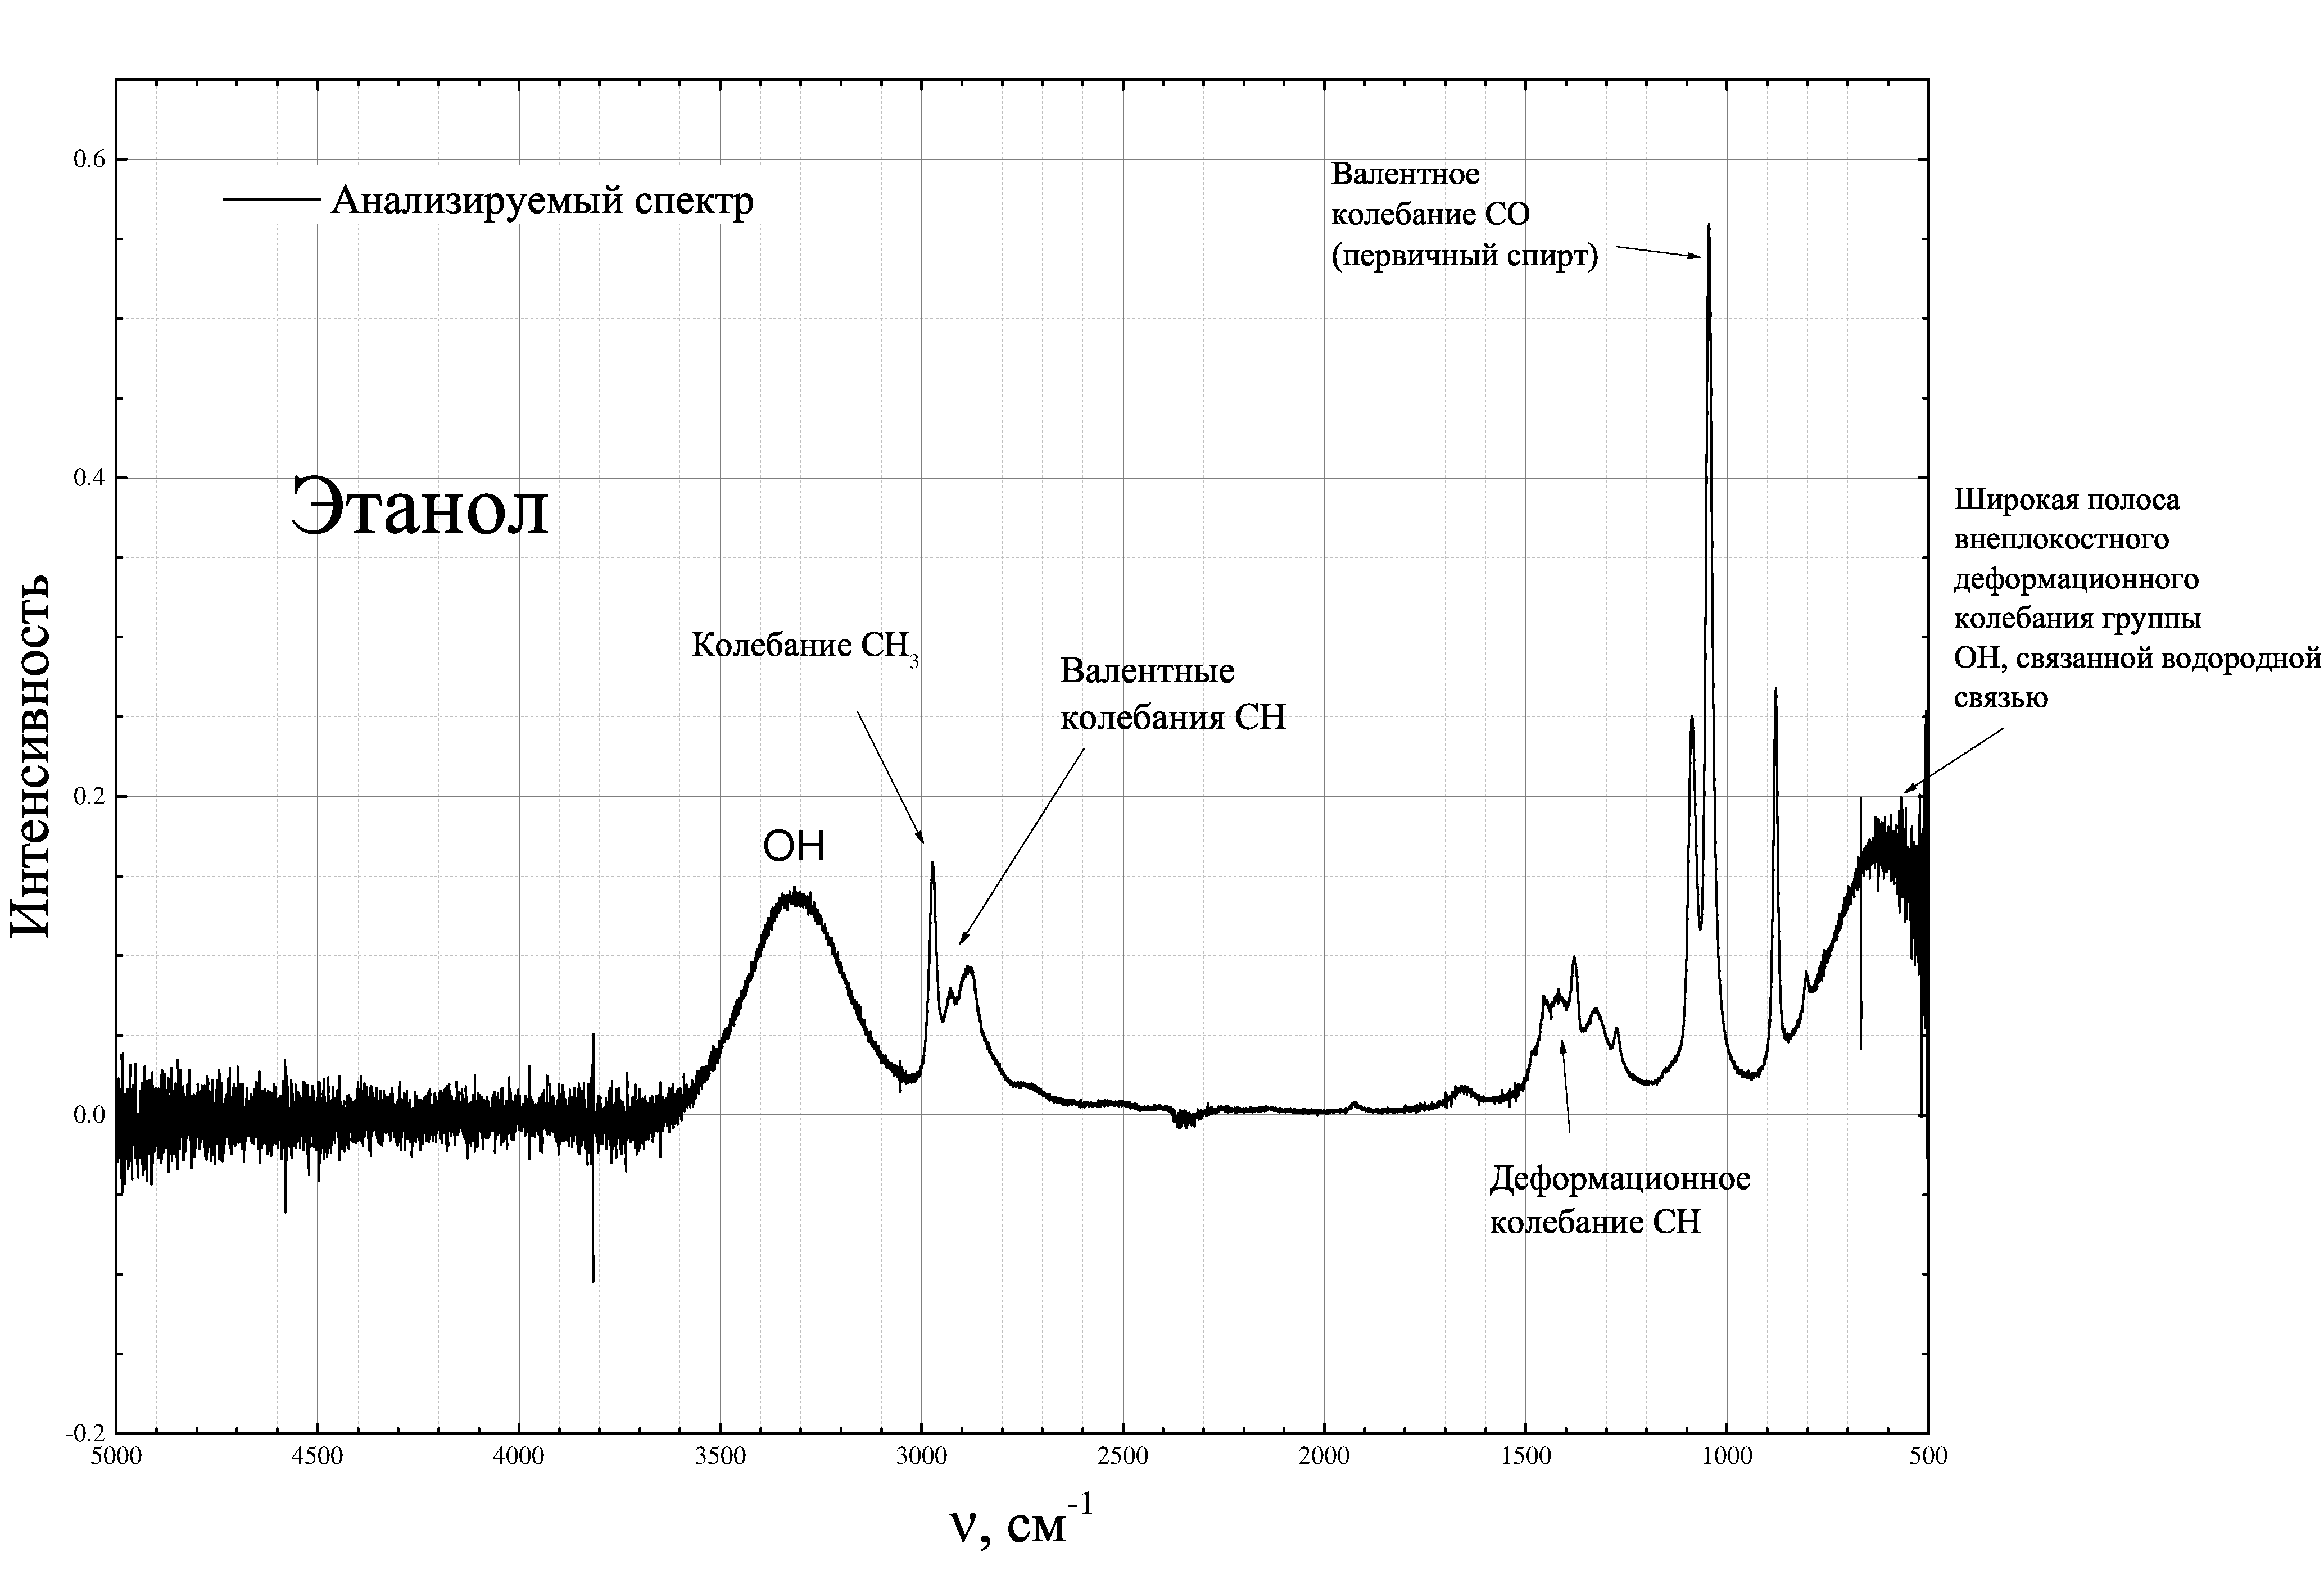
\includegraphics[angle = 90, height=0.95\textheight]{ethanol}
	\caption{Исследуемый спектр (этанол)}
	\label{ethanol}
\end{figure}
\begin{figure}[h!]
	\centering
	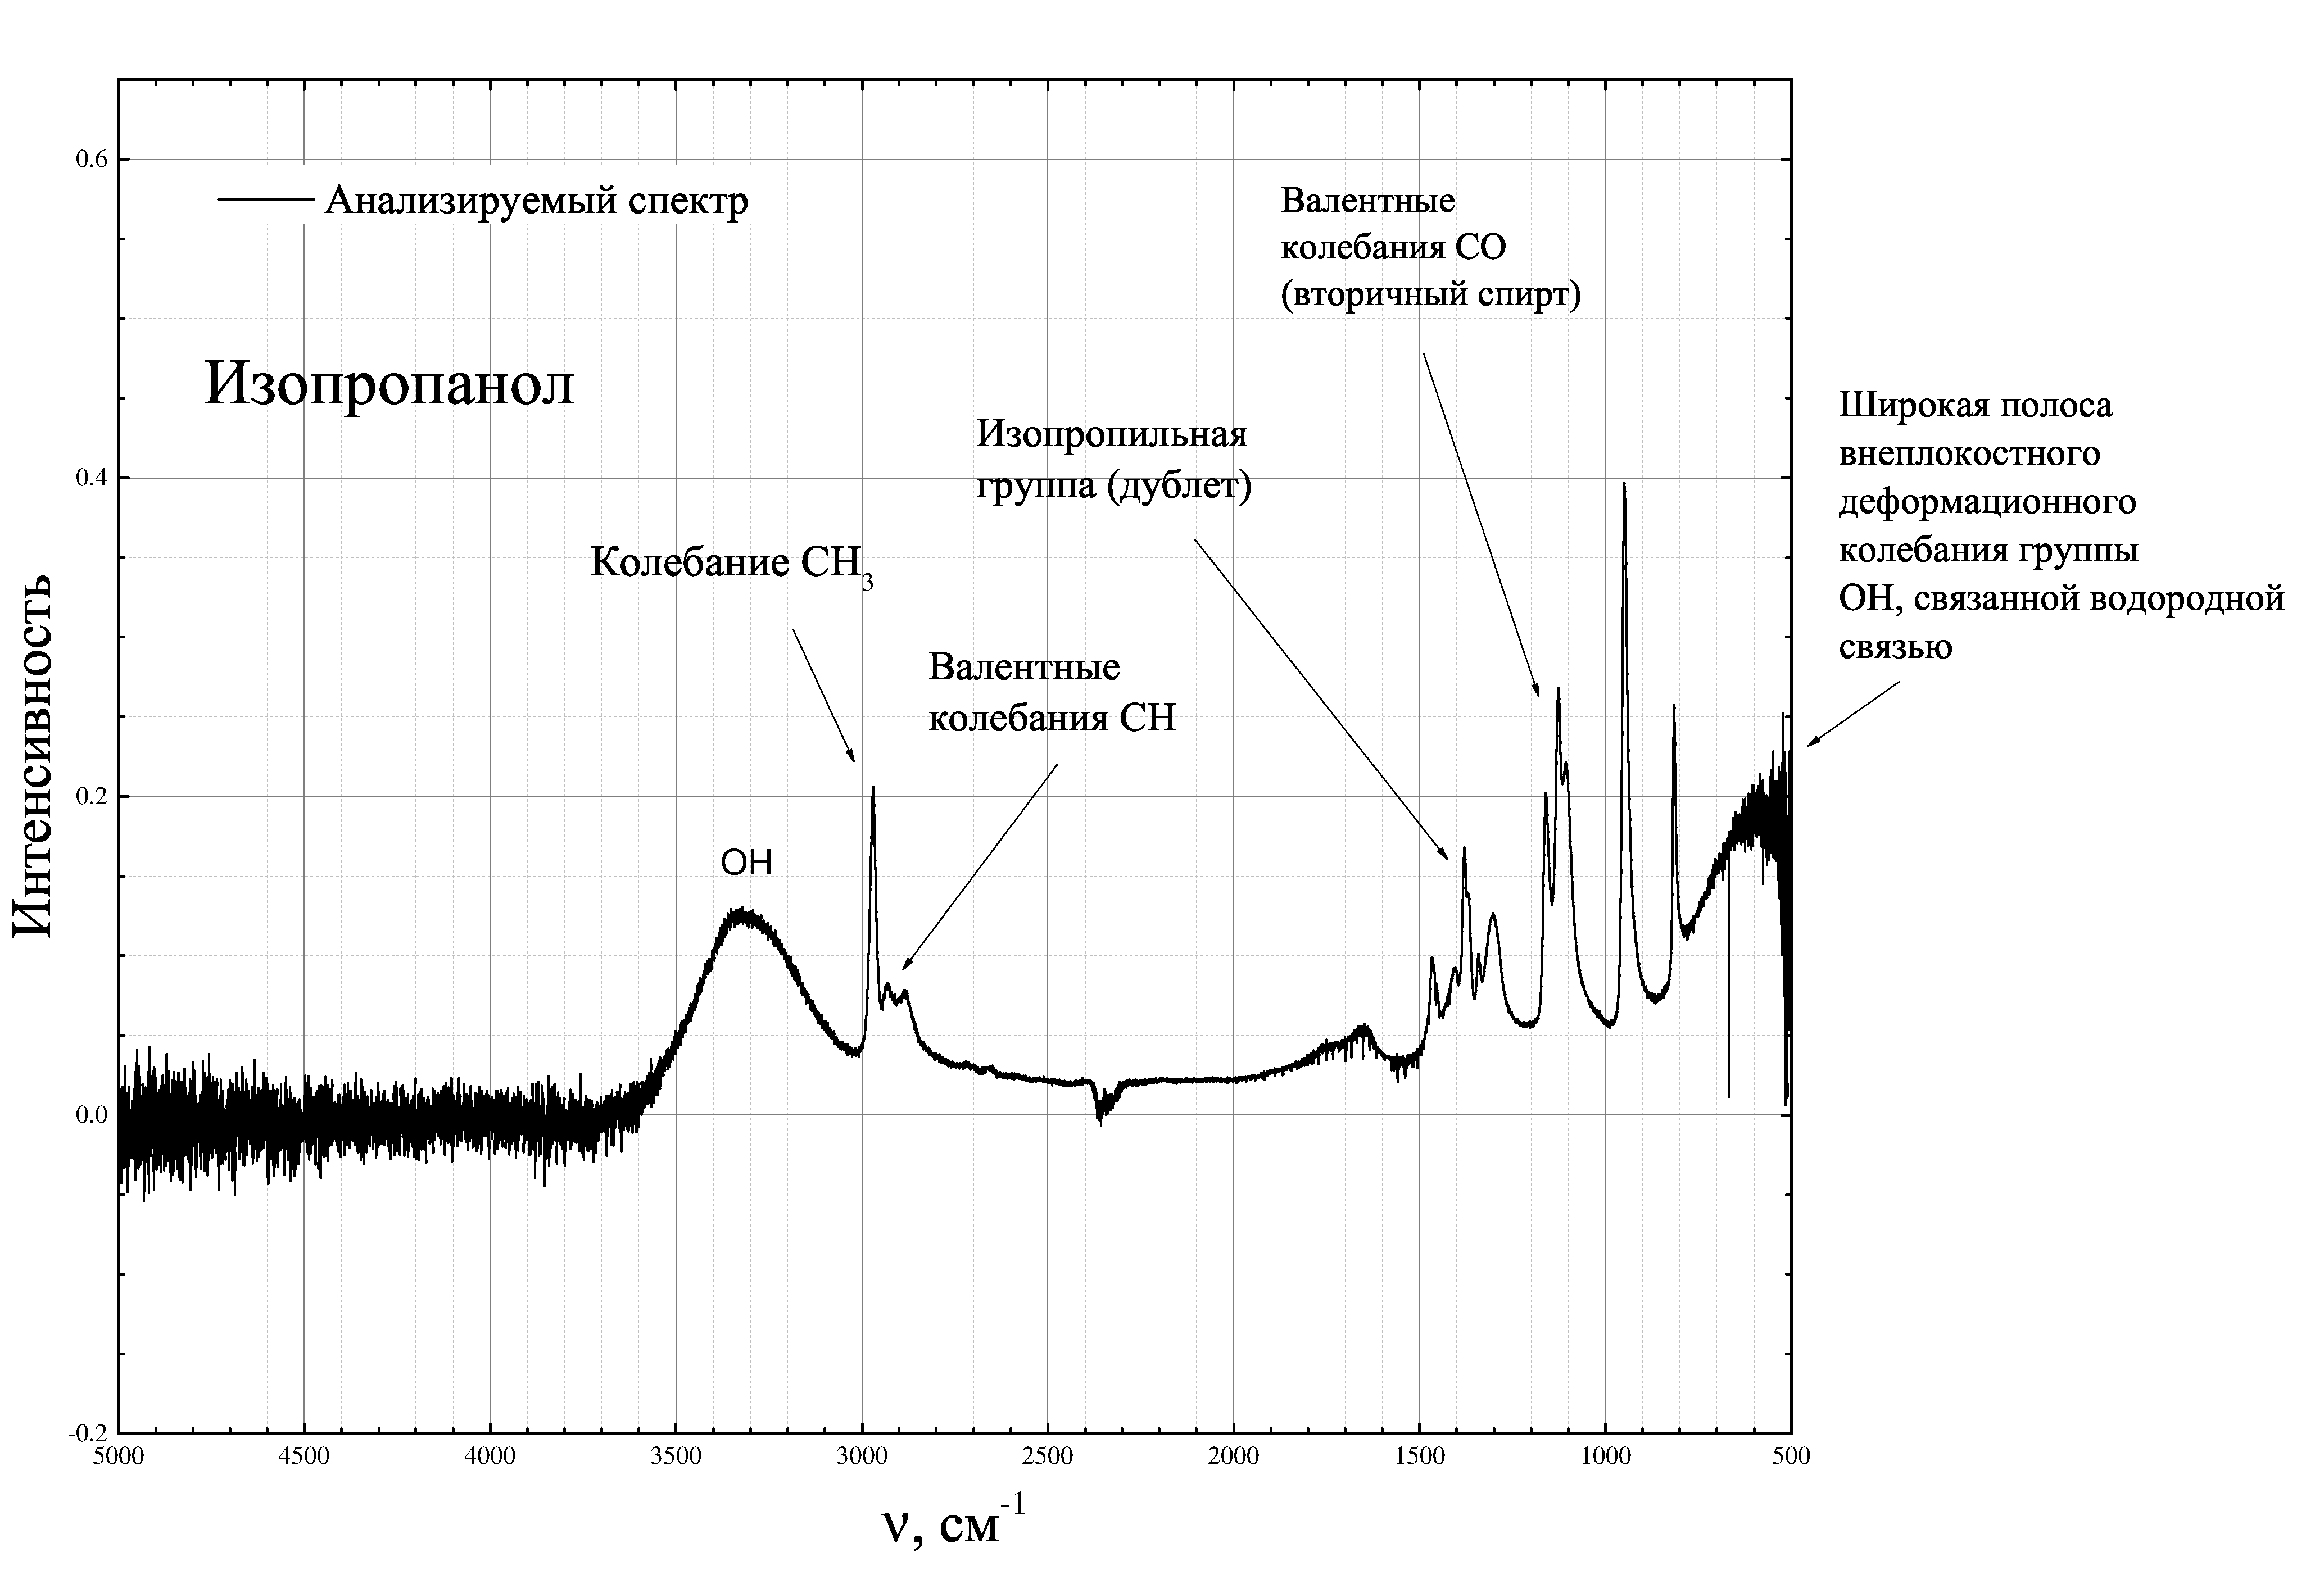
\includegraphics[angle = 90, height=0.95\textheight]{isopropanol}
	\caption{Исследуемый спектр (изопропанол)}
	\label{isopropanol}
\end{figure}
\begin{figure}[h!]
	\centering
	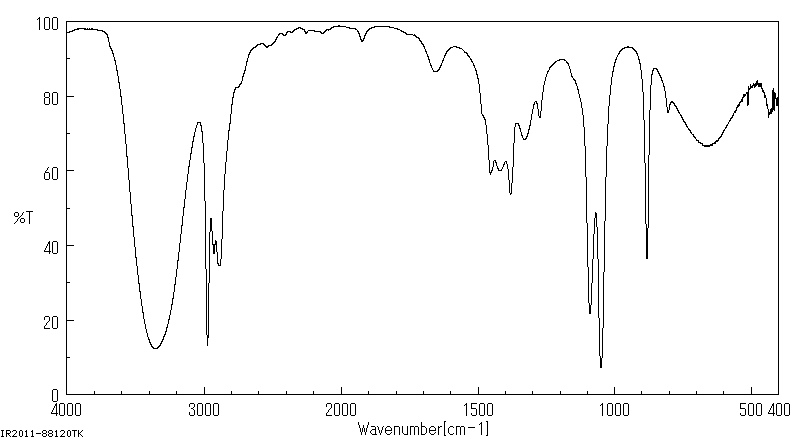
\includegraphics[width=0.9\textwidth]{ethanol_real}
	\caption{ИК-спектр поглощения этанола}
	\label{ethanol_real}
\end{figure}
\begin{figure}[h!]
	\centering
	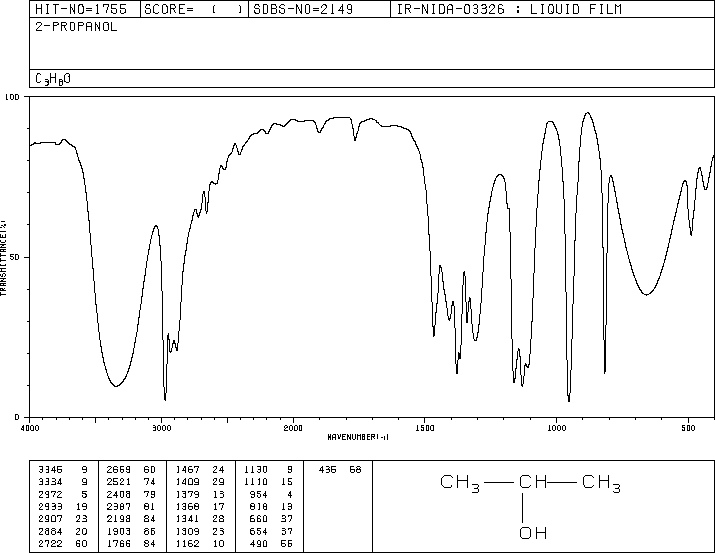
\includegraphics[width=0.9\textwidth]{propanol_real}
	\caption{ИК-спектр поглощения изопропанола}
	\label{propanol_real}
\end{figure}
